%%%%%%%%%%%%%%%%%%%%%%%%%%%%%%%%%%%%%%%%%
% Short Sectioned Assignment LaTeX Template Version 1.0 (5/5/12)
% This template has been downloaded from: http://www.LaTeXTemplates.com
% Original author:  Frits Wenneker (http://www.howtotex.com)
% License: CC BY-NC-SA 3.0 (http://creativecommons.org/licenses/by-nc-sa/3.0/)
%%%%%%%%%%%%%%%%%%%%%%%%%%%%%%%%%%%%%%%%%

%----------------------------------------------------------------------------------------
%	PACKAGES AND OTHER DOCUMENT CONFIGURATIONS
%----------------------------------------------------------------------------------------

\documentclass[paper=a4, fontsize=11pt]{scrartcl} % A4 paper and 11pt font size

% ---- Entrada y salida de texto -----

\usepackage[T1]{fontenc} % Use 8-bit encoding that has 256 glyphs
\usepackage[utf8]{inputenc}
%\usepackage{fourier} % Use the Adobe Utopia font for the document - comment this line to return to the LaTeX default

% ---- Idioma --------

\usepackage[spanish, es-tabla]{babel} % Selecciona el español para palabras introducidas automáticamente, p.ej. "septiembre" en la fecha y especifica que se use la palabra Tabla en vez de Cuadro

% ---- Otros paquetes ----

\usepackage{url} % ,href} %para incluir URLs e hipervínculos dentro del texto (aunque hay que instalar href)
\usepackage{amsmath,amsfonts,amsthm} % Math packages
%\usepackage{graphics,graphicx, floatrow} %para incluir imágenes y notas en las imágenes
\usepackage{graphics,graphicx, float} %para incluir imágenes y colocarlas

% Para hacer tablas comlejas
%\usepackage{multirow}
%\usepackage{threeparttable}

%\usepackage{sectsty} % Allows customizing section commands
%\allsectionsfont{\centering \normalfont\scshape} % Make all sections centered, the default font and small caps

\usepackage{fancyhdr} % Custom headers and footers
\pagestyle{fancyplain} % Makes all pages in the document conform to the custom headers and footers
\fancyhead{} % No page header - if you want one, create it in the same way as the footers below
\fancyfoot[L]{} % Empty left footer
\fancyfoot[C]{} % Empty center footer
\fancyfoot[R]{} % Page numbering for right footer
\renewcommand{\headrulewidth}{0pt} % Remove header underlines
\renewcommand{\footrulewidth}{0pt} % Remove footer underlines
\setlength{\headheight}{13.6pt} % Customize the height of the header

\numberwithin{equation}{section} % Number equations within sections (i.e. 1.1, 1.2, 2.1, 2.2 instead of 1, 2, 3, 4)
\numberwithin{figure}{section} % Number figures within sections (i.e. 1.1, 1.2, 2.1, 2.2 instead of 1, 2, 3, 4)
\numberwithin{table}{section} % Number tables within sections (i.e. 1.1, 1.2, 2.1, 2.2 instead of 1, 2, 3, 4)

\setlength\parindent{0pt} % Removes all indentation from paragraphs - comment this line for an assignment with lots of text

\newcommand{\horrule}[1]{\rule{\linewidth}{#1}} % Create horizontal rule command with 1 argument of height


\usepackage{hyperref}
\usepackage{listings}
\usepackage{xcolor}
\usepackage{caption}
\usepackage{subcaption}
\usepackage{lmodern}
\usepackage{graphicx}
\usepackage{biblatex}
\usepackage{array}
\usepackage{wrapfig}

\definecolor{codegreen}{rgb}{0,0.6,0}
\definecolor{codegray}{rgb}{0.5,0.5,0.5}
\definecolor{codepurple}{rgb}{0.58,0,0.82}
\definecolor{backcolour}{rgb}{0.95,0.95,0.92}
\usepackage[margin=0.7in]{geometry}

\newcolumntype{C}[1]{>{\centering\arraybackslash}p{#1}}
\newcolumntype{L}[1]{>{\raggedright\arraybackslash}p{#1}}
\newcolumntype{R}[1]{>{\raggedleft\arraybackslash}p{#1}}

\lstdefinestyle{mystyle}{
    backgroundcolor=\color{backcolour},   
    commentstyle=\color{codegreen},
    keywordstyle=\color{magenta},
    numberstyle=\tiny\color{codegray},
    stringstyle=\color{codepurple},
    basicstyle=\ttfamily\footnotesize,
    breakatwhitespace=false,         
    breaklines=true,                 
    captionpos=b,                    
    keepspaces=true,                 
    numbers=left,                    
    numbersep=5pt,                  
    showspaces=false,                
    showstringspaces=false,
    showtabs=false,                  
    tabsize=2
}


\title{	
\normalfont \normalsize 
\textsc{\textbf{Metaheurística grupo 2 (2021-2022)} \\ Grado en Ingeniería Informática \\ Universidad de Granada} \\ [25pt] % Your university, school and/or department name(s)
\horrule{0.5pt} \\[0.4cm] % Thin top horizontal rule
\huge Práctica 3 \\
Mínima dispersión diferencial \\ % The assignment title
\horrule{2pt} \\[0.5cm] % Thick bottom horizontal rule
}

\author{José María Ramírez González\\\href{mailto:jmramirez@correo.ugr.es}{jmramirez@correo.ugr.es}} % Nombre y apellidos

\date{\normalsize\today} % Incluye la fecha actual

\begin{document}

\maketitle % Muestra el Título

\newpage %inserta un salto de página

\tableofcontents % para generar el índice de contenidos

\newpage

\section{Descripción del problema}

El problema escogido es el conocido como \textit{mínima dispersión diferencial} o \textit{minimun differential dispersion} en inglés.

En este problema se intenta minimizar la dispersión entre un subconjunto $M$ de elementos de un conjunto $C$. Es un problema \textbf{NP-completo}, por lo que resulta inviable resolverlo de manera óptima en un tiempo decente en casos donde $|C|$ o $|M|$ sean grandes.

Nuestro objetivo es encontrar $M \subset C$, y se nos proporcionarán varios casos, cada uno con un $C$ y un $m =|M|$.
En cada caso nos dan, además, la distancia de un elemento al resto de ellos, tal que podamos calcular el \textit{$\Delta$-value} de cada elemento como $\displaystyle \Delta \text{-value}_i = \sum_{j \in M}d_{ij}\quad \forall \, i \in M$, donde $d_{ij}$ es la distancia del elemento $i$ al elemento $j$.

Para calcular la dispersión, realizamos el siguiente cálculo $disp = max(\Delta\text{-value})-min(\Delta\text{-value})$. Esa sería la dispersión asociada a una posible solución $M$, el máximo de sus $\Delta$-values menos el mínimo de ellos. Así pues, nuestra función a minimizar es esa.

Es importante destacar que la dispersión de cada conjunto solución $M$ depende de cada uno de los elementos $w \in M$ y que, cambiando tan solo uno de ellos, esta puede cambiar radicalmente.

\section{Elementos comunes empleados en la resolución del problema}
Para resolver este problema, hemos implementado los siguientes algoritmos:
\begin{itemize}
\item Un algoritmo \textbf{Greedy}.
\item Un algoritmo de \textbf{Búsqueda local}.
\item Un algoritmo de \textbf{Enfriamiento Simulado (ES)}.
\item Un algoritmo de \textbf{Búsqueda Multiarranque Básica (BMB)}.
\item Un algoritmo de \textbf{Búsqueda Local Reiterada (ILS)}.
\end{itemize}

El código de los algoritmos de la práctica 1, \textit{greedy} y \textit{búsqueda local}, no estará en esta práctica.

Más adelante estudiaremos estos algoritmos, pero antes, vamos a comentar algunos elementos comunes a ambos.

\subsection{Representación de los datos}

Los datos de entrada se nos proporcionan en un fichero con la estructura que podemos apreciar en el listing \ref{lst:estructuraFicheros}.

\begin{lstlisting}[frame=single,caption={Estructura de los ficheros proporcionados},label=lst:estructuraFicheros, captionpos=b]
n m
0 1 value
0 2 value
...
n-2 n-1 value
\end{lstlisting}

Donde $m = |M|$, $n = |C|$ y \textit{value} es el coste de ir de la posición que aparece primero a la posición que aparece en segundo lugar. En nuestro caso, guardaremos esta información en forma de matriz cuadrada $n \times n$, donde rellenamos el triangulo superior y el inferior, para no tener que comprobar índices, y dejaremos 0s en la diagonal principal.

El funcionamiento general de la lectura de los datos sería el representado en el listing \ref{lst:funcionamientoLeerDatos}.

\begin{lstlisting}[frame=single, caption={Generalización de la lectura de los datos},label=lst:funcionamientoLeerDatos, captionpos=b]
archivo = open(archivoConDatos)
n, m = archivo.get(0,1)
matriz = nuevaMatriz(n x n, 0) # Nueva matriz n*n de 0s
for linea in archivo:
    pos1 = linea[0]
    pos2 = linea[1]
    valor = linea[2]
    matriz[pos1][pos2] = valor
    matriz[pos2][pos1] = valor
\end{lstlisting}


\subsection{Representación de la solución}

Para representar los elementos seleccionados, vamos a contar con un vector de tamaño $n$, donde los elementos seleccionados tendrán valor $1$ y los no seleccionados, valor $0$.

Es importante destacar que para que una solución sea válida, el vector solución tiene que tener tantos $1$s como el valor de $m$.

Con este vector y con la matriz de datos podemos calcular la dispersión para una posible solución.


\subsection{Función objetivo}

Nuestro objetivo es minimizar la dispersión de la solución final.
La dispersión se define como la diferencia entre el mayor $\Delta$-value y el menor $\Delta$-value.
El $\Delta$-value está asociado a cada posición seleccionada, de tal forma que $\Delta$-value$_{i} = \sum_{k=0}^{m}datos[i][k]$, es decir, la suma de las distancias de cada elemento seleccionado al resto de elementos seleccionados. Por tanto, nuestra Disp$_i$ sería el mayor de estos valores menos el menor.

A la sumatoria anterior vamos a darle el nombre de \texttt{calcularDvalue}.

Para calcular la dispersión, tan solo tenemos que hacer lo definido en el listing \ref{lst:calcDisp}:

\begin{lstlisting}[frame=single, caption={Cálculo de la dispersión para una posible solución}, captionpos=b, label=lst:calcDisp]
pesosSolucion = []
para seleccion en Solucion: # Donde solucion es un vector
    pesosSolucion += calcularDvalue(seleccion)

ordenar(pesosSolucion)
Dispersion = pesosSolucion.last() - pesosSolucion.first()
\end{lstlisting}

Por lo tanto, nuestro objetivo es buscar una solución que nos minimice la dispersión.



\subsection{Selección de los datos de entrada}

Para seleccionar los datos de entrada, hacemos uso de la librería \textit{os} con la que, introduciendo el nombre de la carpeta donde tenemos todos los archivos con los datos de entrada, nos leerá los nombres de los mismos.

Una vez tengamos los nombres, los ordenamos de menor a mayor con una función que hemos creado y pasamos a ejecutar un bucle que realiza todos los algoritmos para cada archivo.

Podemos encontrar el pseudocódigo en el listing \ref{lst:lecturaArchivos}.

\begin{lstlisting}[frame=single, caption={Versión búsqueda local}, captionpos=b, label=lst:lecturaArchivos]
archivos = leerCarpeta(nombreCarpeta)
ordenarPorNombre(archivos)
para cada archivo en archivos:
    leer(archivo)
    Ejecutar algoritmos
\end{lstlisting}


\subsection{Aleatoriedad en los algoritmos}

Todos los algoritmos implementados en esta práctica utilizan números aleatorios.

Para obtener esta aleatoriedad vamos a hacer uso tanto del paquete \texttt{random} como de \texttt{numpy.random}.

Esto va a provocar que nuestros algoritmos obtengan resultados distintos en cada ejecución.

\subsection{Medición del tiempo de ejecución}

Para medir los tiempos de ejecución de cada algoritmo, hemos hecho uso de la librería \textit{time}, la cual nos proporciona el tiempo de CPU que tarda en ejecutarse una determinada parte del código con una implementación similar a la del listing \ref{lst:tiempoCPU}.

\begin{lstlisting}[frame=single, caption={Tiempo de ejecución de un programa}, captionpos=b, label=lst:tiempoCPU]
tiempoinicio = tiempoActual()

...
#Ejecucion del algoritmo
...

tiempoFinal = tiempoActual()
tiempoEjecucion = tiempoFinal - tiempoInicio
\end{lstlisting}

\subsection{Generador de soluciones}

Al comenzar la ejecución el algoritmo, vamos a necesitar una o varias soluciones iniciales.

Para generar una posible solución, simplemente vamos a generar un vector de tamaño $n$ sin elementos seleccionados y a seleccionar aleatoriamente $m$ elementos de ese vector.
Esa solución será factible.

Podemos ver una implementación de este generador de soluciones en el listing \ref{lst:generarSol}

\begin{lstlisting}[frame=single, caption={Generador de soluciones}, captionpos=b, label=lst:generarSol]
solucion = [0,0,0,0,0,...,0]  # n 0s

indices = seleccionar m elementos de [0,1,...,n-1] aleatoriamente

solucion[indices] = 1

return solucion
\end{lstlisting}

\newpage

\section{Enfriamiento simulado}

Este algoritmo consiste en ir reduciendo la temperatura de nuestro sistema gradualmente conforme avanzamos hacia soluciones mejores.

Vamos a comenzar con una temperatura inicial $T_0$, definida como $\displaystyle T_0 = \frac{\mu \cdot C(S_0)}{-\ln(\phi)}$, donde $\mu$ y $\phi$ son constantes que se proporcionan por parámetros.

Iremos ``enfriando'' el sistema tal que $\displaystyle T_{k+1}= \frac{T_k}{1+ \beta \cdot T_k}$, donde $\displaystyle \beta = \frac{T_0 - T_f}{M\cdot T_0 \cdot T_f}$, siendo $T_f$ la temperatura final y $M$ el número de enfriamientos que deberíamos de realizar para pasar de $T_0$ a $T_f$.

Durante la ejecución del algoritmo, generaremos vecinos de la solución actual según pseudocódigo del listing \ref{lst:generarVec}.

\begin{lstlisting}[frame=single, caption={Generador de vecinos}, captionpos=b, label=lst:generarVec]
indicesSeleccionados = indices(Solucion)
opcionesDisponibles = [1, 2, ..., n-1] - indicesSeleccionados

paraSacar = elegirAleatorio(1, indicesSeleccionados)
paraMeter = elegirAleatorio(1, opcionesDisponibles)

return Int(Solucion, pesosSolucion, paraSacar, paraMeter)
\end{lstlisting}

Como vemos, se hace referencia a la función \texttt{Int}, que es la que usamos en la búsqueda local para realizar el intercambio de elementos seleccionados y no seleccionados.

A su vez, vamos a restringir el número de vecinos que podemos generar entre cada enfriamiento a $10 \cdot n$. Realizaremos lo mismo con el número de vecinos que podemos aceptar, pero limitándolo a $n$.

Tendremos cierta probabilidad de aceptar un resultado peor que el actual, esto nos permitirá ampliar el espacio de búsqueda.
Esta posibilidad se va reduciendo conforme nos acercamos a $T_f$, generando un número aleatorio entre 0 y 1 y comparándolo con la función $\displaystyle e^{-\frac{\Delta C(S)}{T}}$ y si el número es menor o igual que el resultado de la función, aceptamos.

Se puede apreciar que el valor de la función se reduce conforme reducimos la temperatura, ya que si tenemos una $T$ muy pequeña, tendremos un valor muy grande o rozando el 0. Si el valor es muy grande, tenemos que aceptar (ya que $\Delta C(S)$ será negativo, lo que quiere decir que estamos reduciendo la dispersión), mientras que si el valor es muy pequeño habrá muy pocas posibilidades de que ese valor aleatorio sea menor. Vamos a denominar a esto que acabamos de explicar como \texttt{aceptarPeor} para que el pseudocódigo del listing \ref{lst:ES}, que contendrá el funcionamiento del algoritmo, sea más simple.

\begin{lstlisting}[frame=single, caption={Enfriamiento simulado}, captionpos=b, label=lst:ES]
mientras que iters < max_iters y n_exitos != 0:
    n_vecinos = n_exitos = 0
    mientras que n_vecinos < max_vecinos y n_exitos < max_exitos:
        n_vecino++
        iters++
        nueva_sol, nuevos_pesos = generarVecino(sol, pesos_sol)
        incr_f = dispersion(nuevos_pesos) - dispersion(pesos_sol)
        
        si incr_f < 0 o aceptarPeor():
            n_exitos++
            sol = nueva_sol
            pesos_sol = nuevos_pesos         
            if dispersion(pesos_sol) < dispersion(mejor_pesos):
                mejor_sol = sol
                mejor_pesos = pesos_sol
                
    decrementar(T)
return iters, dispersion(mejor_pesos)
\end{lstlisting}


\section{Búsqueda multiarranque básica}

Este algoritmo resulta bastante sencillo, simplemente generamos un número determinado de soluciones iniciales, aplicamos búsqueda local a cada una de ellas y devolvemos la mejor de todas.

Se puede ver su implementación en pseudocódigo en el listing \ref{lst:BMB}.

\begin{lstlisting}[frame=single, caption={Búsqueda multiarranque básica}, captionpos=b, label=lst:BMB]
soluciones = []

for i in num_soluciones:
    soluciones += generarSolucion()

for solucion in soluciones:
    aplicarBL(solucion)

soluciones.ordenar(dispersion(soluciones))

return dispersion(soluciones[0])
\end{lstlisting}


\section{Búsqueda local reiterada (ILS)}

Este algoritmo consiste en generar una solución inicial y aplicar un algoritmo de búsqueda local sobre la misma, optimizando la solución inicial. A partir de aquí, se generarán mutaciones de la mejor solución encontrada hasta el momento, aplicándoles el algoritmo de explotación a cada una de las soluciones mutadas, esperando así obtener mejores soluciones.
Esto se repetirá un número determinado de veces.

El algoritmo de mutación que se usa es similar al de generación de vecinos del listing \ref{lst:generarVec}, simplemente cambiando el hecho de que seleccionaremos el número de valores a mutar, que será $aMutar = \mu \cdot m$, donde $\mu$ es una valor entre 0 y 1 y mínimo se mutará un elemento.

La explotación que se aplique en este algoritmo puede ser cualquiera. En nuestro caso, realizaremos una variante con enfriamiento simulado y otra con la búsqueda local implementada en la práctica 1.

podemos ver la implementación en pseudocódigo del algoritmo en el listing \ref{lst:ILS}.

\begin{lstlisting}[frame=single, caption={Búsqueda local reiterada}, captionpos=b, label=lst:ILS]
mejor_sol = algoritmo(sol) // El algoritmo de explotacion usado

repetir tantas veces como iteraciones-1:
    sol = mutar(mejor_sol)
    sol = algoritmo(sol)
    
    si dispersion(sol) < dispersion(mejor_sol):
        mejor_sol = sol

return dispersion(mejor_sol)
\end{lstlisting}

\newpage

\section{Desarrollo y uso del software}

En esta sección vamos a comentar cómo hemos desarrollado el software para la práctica, a la vez que indicaremos cómo ejecutar el mismo.


\subsection{Implementación}

A la hora de implementar ambos algoritmos, hemos optado por usar \textit{Python} debido a la sencillez del código, la simplicidad de uso, unos tiempos de ejecución decentes (más lentos que si usamos un lenguaje como \textit{C}, pero correctos para este tipo de software) y, lo más importante, las librerías disponibles y el fácil manejo de tipos de datos como las listas y las matrices.

Todos los algoritmos están escritos en el mismo programa, por lo que no nos tendremos que preocupar de ejecutar varios archivos, tan solo de descomentar y comentar las líneas convenientes si nos queremos limitar a ejecutar un solo algoritmo.

Junto con la memoria, incluiremos un archivo de requisitos en formato \textit{.txt}, de forma que se pueda hacer uso de \textit{pip} para instalar las librerías pertinentes, aunque a excepción de \textit{NumPy}, las otras que usamos vienen instaladas por defecto, por lo que sólo tendríamos que instalar esta.

Es importante destacar que el software nos guardará parte de los resultados para cada archivo, dejándolos en \texttt{./data/<algoritmo>}, con el formato que se observa en el listing \ref{lst:formatoResults}.

\begin{lstlisting}[frame=single, caption={Formato de los archivos para guardar la evolución de los algoritmos}, captionpos=b, label=lst:formatoResults]
Archivo     Tiempo, Dispersion
.....
Archivo     Tiempo, Dispersion
\end{lstlisting}

\subsection{Manual de uso}

Para ejecutar correctamente el ejecutable (\textit{.py}), previamente tenemos que hacer uso de \textit{pip} para instalar los requisitos proporcionados en el archivo \textit{requirements.txt}, en nuestro caso, bastará con instalar \textit{numpy}.
Esto se puede realizar con el comando \texttt{pip install -r requirements.txt} o, en su defecto, si prescindimos del archivo \textit{requirements.txt}, con \texttt{pip install numpy}.

Una vez instalado, tenemos que asegurarnos de comprobar que tenemos en una carpeta localizada los archivos a leer y \textbf{solo} esos archivos, ya que el programa no realiza comprobación sobre los archivos que lee. Esta carpeta se la pasaremos por parámetros al momento de ejecución.

Ahora podemos pasar a ejecutar el archivo con el comando \texttt{python3 <nombreArchivo>.py <ruta carpeta datos>}.

Podremos observar los resultados en tiempo real de los valores medios de tiempo y dispersión para todos los algoritmos y a su vez, se guardarán en el archivo \textit{./data/nombreAlgoritmo}.

\newpage

\section{Experimentos realizados y análisis de resultados}


Vamos a separar esta sección en varias más pequeñas, intentando comprender mejor lo que estamos haciendo en cada parte.

Las diferentes secciones serán:

\begin{itemize}
\item Comparativa de los algoritmos de arranque simple (Greedy, BL y \textit{ES}).
\item Comparativa de los algoritmos de búsqueda para \textit{ILS}.
\item Comparativa de los algoritmos de arranque múltiple (\textit{BMB}, \textit{ILS}).
\item Comparativa de los mejores algoritmos simples y múltiples relativos a esta práctica.
\item Resultados generales de tiempo y desviación media de las pruebas realizadas.
\item Gráficas para observar características de interés.
\item Conclusión general sobre eficiencia en tiempo y resultado de los algoritmos probados.
\end{itemize}

A su vez cabe destacar que para facilitar la comprensión, vamos a usar el término ``multiarranque'' o ``arranque múltiple'' para referirnos a algoritmos tanto de búsqueda iterativa como a aquellos que serían multiarranques propiamente dicho, es decir, usaremos ``multiarranque'' para referirnos tanto a \textit{ILS} como a \textit{BMB}.

\subsection{Comparativa de los algoritmos de arranque simple}

Vamos primero a expresar la tabla con los resultados de desviación y tiempo obtenido de estos algoritmos. Podemos verla en la figura \ref{tab:compSimple}.

\begin{figure}[H]
    \centering
    \begin{tabular}{|c|c|c|}
        \hline
        Algoritmo & \textbf{Desviación} & \textbf{Tiempo}\\
        \hline
        \textbf{Enfriamiento simulado} & 54,85 & 1,01E+00\\
        \hline
        \textbf{Greedy} & 80,32 & 1,42E-02\\
        \hline
        \textbf{BL} & 58,12 & 2,77E-01\\
        \hline
    \end{tabular}
    \caption{Resultados de tiempo y desviación de los algoritmos de arranque simple}
    \label{tab:compSimple}
\end{figure}

Como vemos, el enfriamiento simulado está muy a la par con la búsqueda local, siendo el primero ligeramente mejor en la desviación obtenida, pero un tanto peor en tiempo de ejecución.
Esta diferencia de resultados no deberá notarse demasiado en la práctica, en cambio, la diferencia de tiempo si debería ser más perceptible, resultando, a la hora de ejecutarlo, mucho más lento el enfriamiento simulado que la búsqueda local.

Usar uno u otro dependerá en gran medida de la precisión requerida para los resultados y el tiempo del usuario.

\subsection{Comparativa de los algoritmos de búsqueda para \textit{ILS}}

Puesto que hemos realizado dos versiones del \textit{ILS}, una con búsqueda local y otra con enfriamiento simulado, vamos a comparar estas dos en esta sección y usaremos la mejor para el resto de comparativas del \textit{ILS}.

Podemos ver la tabla obtenida en la figura \ref{tab:compILS}.

\begin{figure}[H]
    \centering
    \begin{tabular}{|c|c|c|}
        \hline
        Algoritmo de búsqueda & \textbf{Desviación} & \textbf{Tiempo}\\
        \hline
        \textbf{ES} & 41,47 & 1,06E+01\\
        \hline
        \textbf{BL} & 12,15 & 2,17E+00\\
        \hline
    \end{tabular}
    \caption{Comparativa de las dos implementaciones de \textit{ILS} realizadas}
    \label{tab:compILS}
\end{figure}

para nuestra sorpresa, el \textit{ILS} ejecutando búsqueda local resulta muchísimo mejor, tanto en tiempo como en resultado obtenido, que el de enfriamiento simulado, por lo que seguiremos el resto de pruebas con este.

\subsection{Comparativa de los algoritmos de arranque múltiple}

Dado que en el subapartado anterior quedó claro, a la vista de los resultados, que el \textit{ILS} que implementaba la búsqueda local resultaba muy superior al de enfriamiento simulado, vamos a comparar el \textit{ILS-BL} con \textit{BMB}.

En la figura \ref{tab:compMult} podemos ver la desviación y el tiempo de ejecución medios.

\begin{figure}[H]
    \centering
    \begin{tabular}{|c|c|c|}
        \hline
        Algoritmo & \textbf{Desviación} & \textbf{Tiempo}\\
        \hline
        \textbf{BMB} & 76,40 & 2,75E+00\\
        \hline
        \textbf{ILS-BL} & 12,15 & 2,17E+00\\
        \hline
    \end{tabular}
    \caption{Comparativa de los algoritmos de arranque múltiple}
    \label{tab:compMult}
\end{figure}

Podemos observar claramente que \textit{BMB} tiene unos resultados más parecidos a un algoritmo voraz (cuyo resultado podemos observar si volvemos a observar la figura \ref{tab:compSimple}). El orden de tiempo es similar al \textit{ILS-BL}, aunque de media tarda un tanto más, poco, pero perceptible.

En resumen, el algoritmo \textit{BMB} no se puede comparar con el \textit{ILS-BL}, siendo este último bastante superior.

\subsection{Comparativa de los mejores algoritmos simples y múltiples relativos a esta práctica}

Siendo los mejores algoritmos el de enfriamiento simulado y el \textit{ILS-BL}, vamos a estudiar la desviación y tiempo de los mismos, que podemos ver en la figura \ref{tab:simYComp}

\begin{figure}[H]
    \centering
    \begin{tabular}{|c|c|c|}
        \hline
        Algoritmo & \textbf{Desviación} & \textbf{Tiempo}\\
        \hline
        \textbf{Enfriamiento simulado} & 54,85 & 1,01E+00\\
        \hline
        \textbf{ILS-BL} & 12,15 & 2,17E+00\\
        \hline
    \end{tabular}
    \caption{Comparativa de los mejores algoritmos de esta práctica}
    \label{tab:simYComp}
\end{figure}

Como se puede observar, a nivel de tiempo están bastante igualados rondando el orden de pocos segundos de media. No obstante, a nivel de desviación, se aprecia un abismo bastante destacable entre ambos, resultando mucho mejor el \textit{ILS-BL}.

Esta comparativa nos sirve para fijar que, en general, un algoritmo de arranque múltiple va a dar mejores resultados que uno de arranque simple, si está bien diseñado e implementado. Esto supondrá una penalización en el tiempo de ejecución, en nuestro caso, muy pequeña.

\subsection{Resultados generales de tiempo y desviación media de las pruebas realizadas}

En la figura \ref{tab:compTotal} podemos observar los resultados de tiempo y desviación de todos los algoritmos de interés. Hemos ordenado los algoritmos por desviación.

\begin{figure}[H]
    \centering
    \begin{tabular}{|c|c|c|}
        \hline
        Algoritmo & \textbf{Desviación} & \textbf{Tiempo}\\
        \hline
        \textbf{Greedy} & 80,32 & 1,42E-02\\
        \hline
        \textbf{BMB} & 76,40 & 2,75E+00\\
        \hline
        \textbf{BL} & 58,12 & 2,77E-01\\
        \hline
        \textbf{ES} & 54,85 & 1,01E+00\\
        \hline
        \textbf{ILS-ES} & 41,47 & 1,06E+01\\
        \hline
        \textbf{ILS-BL} & 12,15 & 2,17E+00\\
        \hline
    \end{tabular}
    \caption{Resultados de tiempo y desviación de los algoritmos de arranque simple}
    \label{tab:compTotal}
\end{figure}

En esta figura podemos apreciar varias cosas:

\begin{itemize}
    \item El pésimo desempeño de \textit{BMB}, siendo tan solo ligeramente superior al algoritmo voraz implementado en la primera práctica.
    \item Las dos versiones de \textit{ILS}, siendo las que mejores resultados aportan y reforzando la conclusión que alcanzamos en el subapartado anterior: los multiarranque suelen tener un mejor desempeño que los de arranque simple.
    \item El potencial del arranque múltiple, que consigue mejorar el desempeño del \textit{ES}, pasando la desviación de 55 a 41 con una ligera penalización en el tiempo de ejecución.
\end{itemize}


\subsection{Gráficas para observar características de interés}

En este apartado vamos a mostrar algunas gráficas que nos van a facilitar la comprensión de las conclusiones alcanzadas en los subapartados anteriores, a la vez que nos permitirán apreciar detalles que hemos pasado por alto analizando tan solo la desviación y tiempo de ejecución medios.

Para comenzar, vamos a ver la dispersión por archivo de todos los algoritmos probados en esta práctica. En la figura \ref{fig:dispTodos} tenemos la gráfica correspondiente.

\begin{figure}[H]
    \centering
    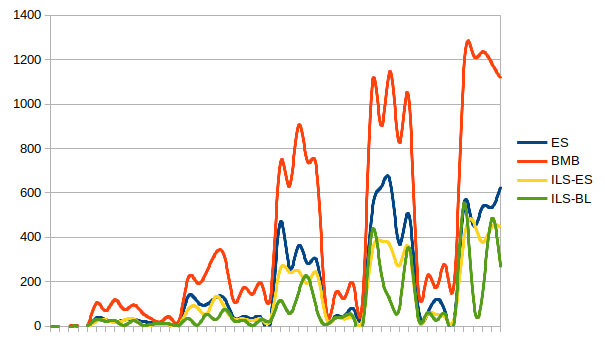
\includegraphics[width=0.65\textwidth]{"data/disp_todos.png"}
    \caption{Dispersión por archivo de todos los algoritmos}
    \label{fig:dispTodos}
\end{figure}

Como vemos, el \textit{BMB} destaca sobre el resto, por lo que vamos a observar la figura \ref{fig:disp_mejores}, similar a la anterior pero quitando el \textit{BMB}, en la que podremos apreciar mejor la evolución del resto de algoritmos.

\begin{figure}[H]
    \centering
    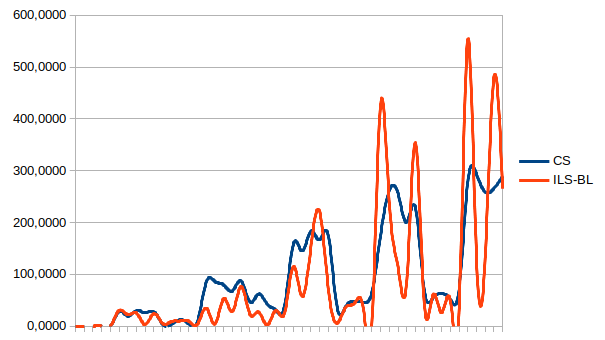
\includegraphics[width=0.65\textwidth]{"data/disp_mejores.png"}
    \caption{Dispersión por archivo de todos los algoritmos a excepción del \textit{BMB}}
    \label{fig:disp_mejores}
\end{figure}

En general, si vemos las dos figuras anteriores, podemos apreciar que todas siguen la misma tendencia: se disparan las dispersiones cuando aumentamos $m$ sin aumentar $n$.
En algunos algoritmos este aumento brusco de la dispersión se nota muchísimo más, como es el caso de \textit{BMB}, mientras que en otros se aprecia menos.

En esta última figura, la \ref{fig:disp_mejores}, se puede ver que las distintas implementaciones de \textit{ILS} tienen mejores resultados que el enfriamiento simulado, como ya comentamos previamente. Esto es así en prácticamente la totalidad de los archivos de prueba.


Vamos ahora a visualizar una gráfica en la figura \ref{fig:tiempoTodos} para apreciar el tiempo de ejecución por archivo de los algoritmos.

Cabe destacar que el tiempo lo estamos expresando en escala logarítmica, ya que puede variar enormemente entre los primeros archivos y los últimos.

\begin{figure}[H]
    \centering
    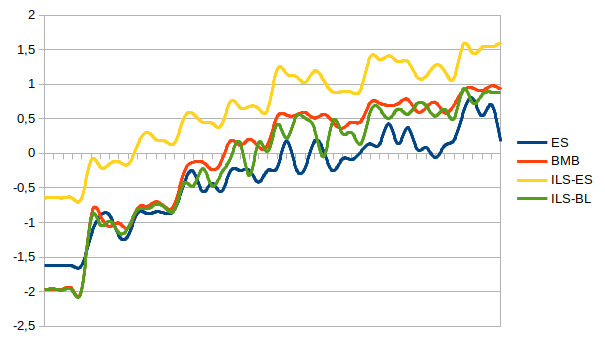
\includegraphics[width=0.65\textwidth]{"data/tiempo_todos.png"}
    \caption{Tiempo por archivo de todos los algoritmos}
    \label{fig:tiempoTodos}
\end{figure}

Podemos observar que el que más tarda de todos es el \textit{ILS-ES} con diferencia, estando los otros 3 bastante parejos.
Sin embargo y si nos fijamos muy de cerca, se puede apreciar que el crecimiento es ligeramente menor en enfriamiento simulado que en los multiarranques. Esto nos indica que los multiarranques, por norma general, van a ser menos tolerantes al tamaño de la muestra, es decir, la pendiente del crecimiento en función del número de muestras es mayor.



\newpage

\subsection{Conclusión general sobre los algoritmos estudiados}

Después de este estudio de los resultados obtenidos experimentalmente, sólo nos queda llegar a una conclusión.

Recapitulando, tenemos que los resultados obtenidos suelen ser mejores en los multiarranques que en los genéticos, pero los tiempos de ejecución son algo mayores en estos últimos.

También tenemos que algunos modelos multiarranque no tienen por qué ser buenos, como es el caso del \textit{BMB}.

Hemos concluido también que el \textit{ILS} funciona mejor con búsqueda local que con enfriamiento simulado.

También podemos decir que el algoritmo de búsqueda local no queda descartado de una lista de posibles resoluciones a este problema, ya que tiene unos valores bastante buenos, tanto en tiempo como en desviación, pudiendo dar algunos resultados incluso mejores que algunos multiarranques.


Dicho esto, tenemos que los algoritmos multiarranque suelen proporcionar un resultado de mayor calidad que el resto, no obstante si el tiempo es un factor crítico, no sería problema optar por usar un algoritmo como sería enfriamiento simulado o búsqueda local, ya que hemos visto que estos tienen un tiempo de ejecución menor y los resultados no son tan malos como para quedar descartados por completo.








\end{document}